% ==========================
% # Sala do \acrshort{neeec}          #
% ==========================

\subsection{Sala do Núcleo}

A organização da sala do Núcleo, para que esta pudesse ser o local privilegiado de trabalho dos membros do \acrshort{neeec} foi, desde cedo, um dos principais objetivos pelo qual trabalhámos. Aproveitando a chegada do computador oferecido pela HP como patrocínio ao \acrshort{ene3} no dia a seguir à tomada de posse, reformulámos completamente a organização da sala para poder colocar o computador num local adequado, resultando na organização da sala que existiu até ao fim do mandato e que se pode consultar na figura \ref{fig:salaneeec}.

\begin{figure}[ht]
\centering
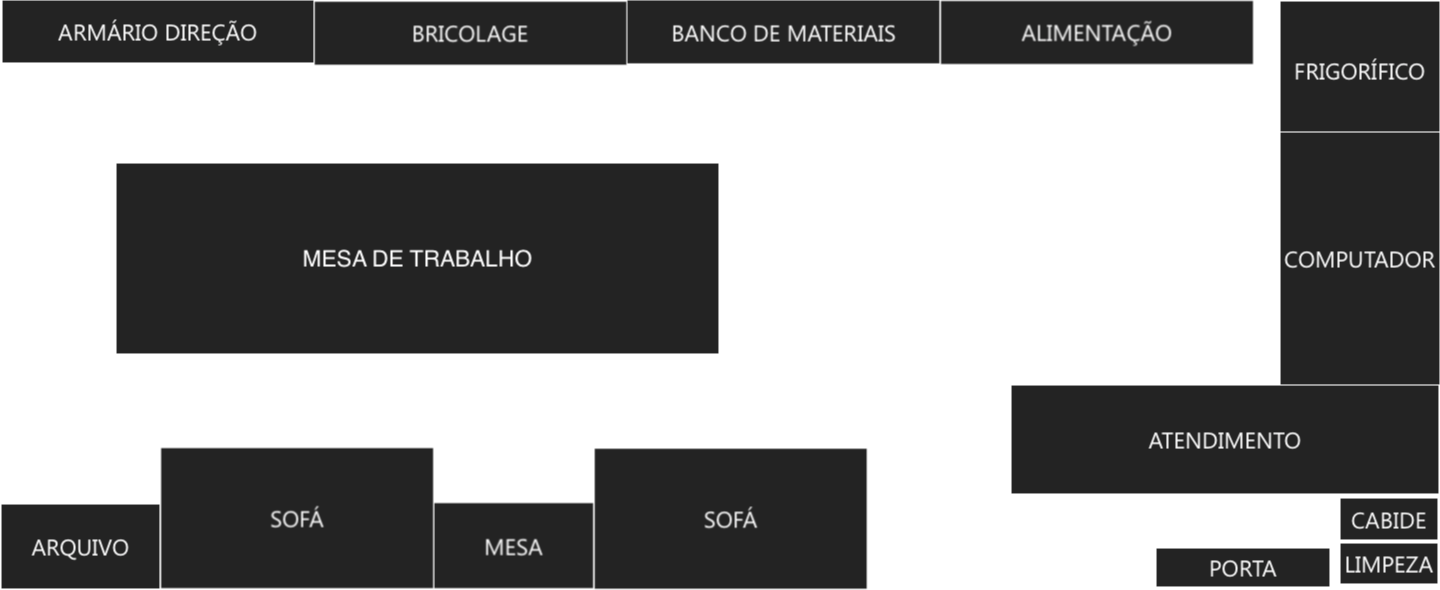
\includegraphics[width=\textwidth]{imagens/salaneeec.png}
\caption{Mapa da Sala do NEEEC.}
\label{fig:salaneeec}
\end{figure}

O nosso objetivo foi criar três espaços principais na sala: o de atendimento ao público (secretária que faz de balcão a quem entra), o espaço de trabalho interno (secretária das reuniões bem como secretária onde se encontra o PC e onde está todo o material de escritório necessário) e espaço de conforto (sofás).

De seguida, após conversações com o Vice-Diretor do Departamento responsável pela gestão do edifício, foi possível trocar todas as cadeiras danificadas da sala por cadeiras novas, oferecidas pelo \acrshort{deec}. Foi também possível, com a ajuda do Departamento, fazer uma puxada de luz para dentro da sala fazendo com que a iluminação passasse a ser controlada dentro da sala e também acabar a obra, iniciada há vários anos atrás, para que pudesse haver tomadas na parede lateral. Por sua vez, foram ainda acrescentados vários pontos de eletricidade nas paredes horizontais da sala e foi feita uma instalação para que a mesa de reuniões dispusesse de cerca de 12 pontos de eletricidade. Foi também necessário arranjar as tampas do chão, algo que estava em elevado estado de degradação. Após a chegada do termoventilador foi necessário também fazer a devida eletrificação do mesmo para ele poder ficar preso na parede.

No que toca à organização dos armários foi criado o armário da Direção, com acesso restrito, para que o cofre ficasse resguardado de forma mais segura e para poder ser guardado o material mais valioso do Núcleo. Todos os armários foram reorganizados e passou a haver identificação sobre o conteúdo dos armários nas suas portas. Algo que foi sempre importante para nós foi que todos os membros do Núcleo facilmente chegassem à sala do Núcleo e pudessem saber onde estavam as coisas pelo que a colocação de sinalética foi essencial. Foi ainda criada uma área para os pelouros e eventos grandes, no armário de arquivo, para que fosse guardado todo o material necessário. Por sua vez, todo o material documental antigo do Núcleo foi catalogado e guardado nos locais corretos. Foi ainda criado um arquivo de cartazes organizado e separado pelos vários anos de mandato.

Como esta é a sala de uma família que trabalha junta diariamente, decidimos colocar fotos de todos os mandatos anteriores que conseguimos na parede deixando assim um retrato das gerações que nos antecederam sempre presente.

De realçar também que o Departamento nos ofereceu um quadro branco novo bem como dois quadros de cortiça que permitiram uma maior área para escrever tudo o que era necessário durante o nosso trabalho.

Fica por fazer a pintura da sala do Núcleo, algo prometido pelo Departamento mas que ainda não foi feito por restrições da Universidade, bem como o arranjo do chão, que já apresenta vários problemas em vários pontos da sala.